\section{방법}
\label{sec:methods}

공식 텔레메트리를 수집하고, 공통 시간축과 지도 좌표축 위에서 네
종류의 STDB 객체로 재구성한다. 네 객체는 이동하는 팀, 동적
안전/블루존, 공간 이벤트, 페이즈 구간이다. 튜토리얼/훈련장 경기와
소수의 비정상 텔레메트리를 제외한 뒤, 그래프 구성이 가능한 경쟁
경기 21,824개를 사용하였다. 재구성한 존 변화 구간을 분석 페이즈
1--8로 인덱싱하고, 예측 기준 페이즈는 1--7로 둔다.
구현상 STDB는 팀 상태, 존, 이벤트, 팀-페이즈, 간선 릴레이션으로
구체화된다. 팀 상태는 경기, 팀, 페이즈, 시간, 좌표, 생존 여부를 담고,
존은 중심, 반경, 시작/종료 시점을 담으며, 이벤트는 위치와 공격/피해 팀 및
이벤트 유형을 기록한다. 팀-페이즈와 간선 릴레이션은 각각 특징/목표값과
출발 팀, 도착 팀, 관계 유형, 가중치를 담아 모델 입력 행과 그래프로 변환된다.

\begin{figure}[htbp]
\centering
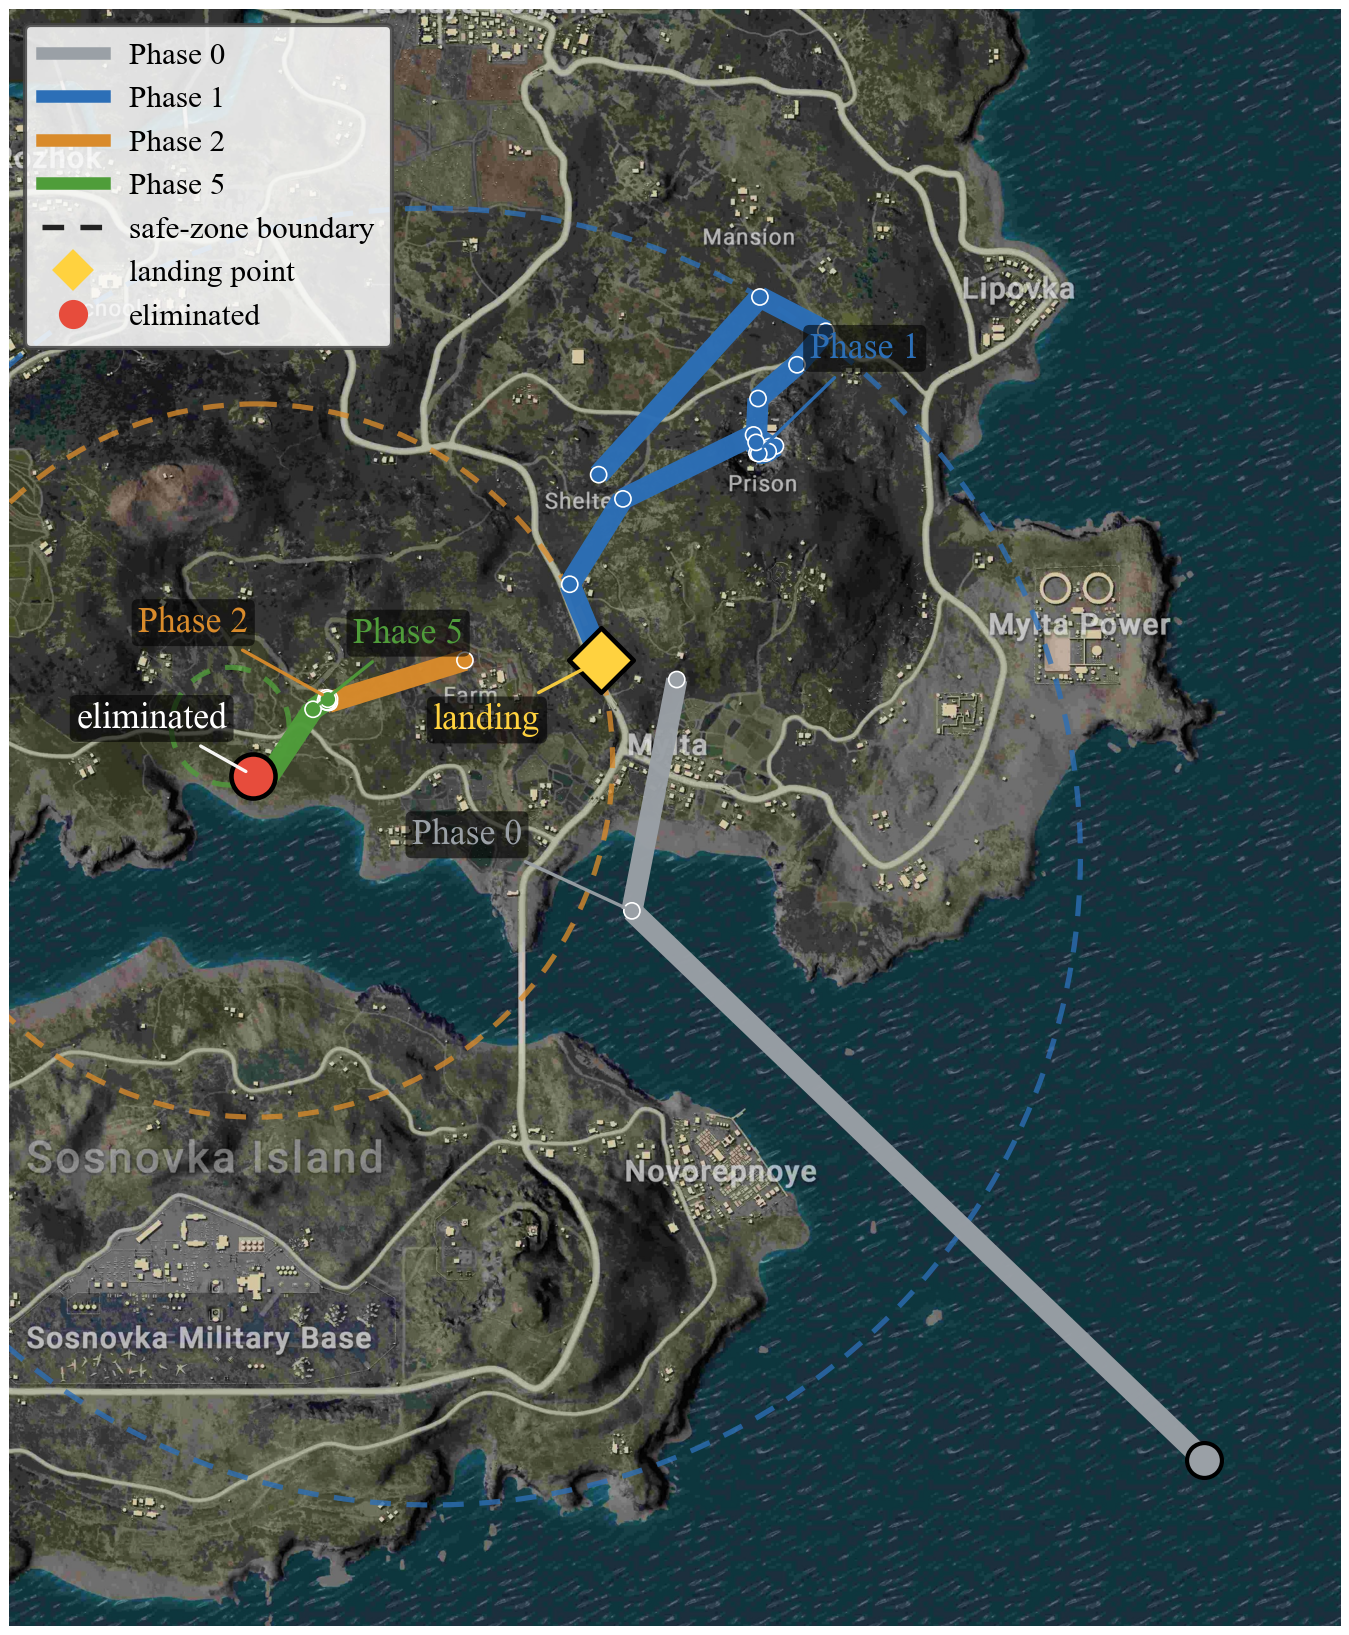
\includegraphics[width=0.88\linewidth]{figures/team_phase_feature_example.png}
\caption{팀-페이즈 STDB 예시. 팀 centroid 궤적을 페이즈별 안전 구역
경계와 정렬하고, landing point, phase movement, elimination point를
하나의 페이즈 인덱스 공간 이력으로 표현한다.}
\label{fig:team-phase-feature-example}
\end{figure}

\paragraph{팀-페이즈 특징.}
모델링 단위는 \((m,i,k)\), 즉 경기 \(m\), 팀 \(i\), 페이즈 \(k\)이다.
각 행은 한 팀의 페이즈 내 이동 궤적, 존 노출, 교전, 상태, 준비도를
요약한다. 표~\ref{tab:feature-sources}에서는 모델 입력의 원천을 기존
텔레메트리 집계와 STDB 시공간 표현으로 나눈다.
\(d\)는 표현 ablation에서 HGB가 사용한 tabular 입력 수이다.
DynamicSTGNN은 같은 원천에서 중복 페이즈 항목과 비수치 표현을 정리한
66개 정규화 수치 노드 특징을 사용한다. 따라서 표의 결합 표현
\(d=72\)와 DynamicSTGNN의 \(F=66\)은 같은 원천을 서로 다른 입력 관점으로
정리한 값이다. STDB 시공간 단독 표현의 16개 변수 중 \(phase\_idx\)는
기존 집계에도 포함되는 공통 cut index이므로, 결합 표현에서는 신규 STDB
변수 15개만 추가된다.

\begin{table}[htbp]
\centering
\caption{기존 텔레메트리 집계와 STDB 시공간 표현의 구분.}
\label{tab:feature-sources}
\scriptsize
\setlength{\tabcolsep}{2.5pt}
\begin{tabular}{p{0.18\linewidth}p{0.22\linewidth}rp{0.42\linewidth}}
\toprule
구분 & 특징군 & \(d\) & 대표 특징 \\
\midrule
기존 집계 & 경기/팀 상태, 교전, 준비도 & 57 &
페이즈 길이, 생존 팀/플레이어 수, 체력, 차량, 팀 분산, 피해량, 기절,
처치, 교전 상대, 아이템, 회복/부스트 \\
STDB 시공간 단독 & 궤적, 존/적 노출 & 16 &
페이즈 인덱스, 팀 centroid 이동 거리, 순변위, 속도, 회전 시점, 안전 구역 방향 정렬,
진입 시점, 경계 거리, 블루존 밖 체류 비율, 주변 적 밀도, 최근접 적 거리 \\
결합 표현 & 기존+STDB 시공간 & 72 &
기존 집계와 STDB 궤적/노출 특징을 결합하되, 공통 페이즈 인덱스를 한 번만
센 탈락 위험 예측 입력 \\
\bottomrule
\end{tabular}
\end{table}

팀 위치는 생존 팀원의 centroid로 계산하고, 팀 분산과 최근접 적 관련
변수는 분산된 squad 상황을 보완한다. 모든 특징은 해당 페이즈 내부
관측치에서만 계산하며, 특징별 고정 상수로 스케일링한다. 피해량, 아이템
획득, 교전 이벤트 횟수처럼 드물게 큰 값이 나타나는 변수는 로그 압축한다.
DynamicSTGNN의 각 팀-페이즈 노드는 이 원천들을 정규화한 66차원 벡터로
표현된다.
그림~\ref{fig:team-phase-feature-example}에서는 이 행 단위 표현이 포착하는
공간적 관점을 보여준다.

\paragraph{동적 팀 그래프.}
각 페이즈에 대해 가중 heterogeneous graph
\(G_k=(V_k,X_k,\{A_k^r\}_{r\in R})\)를 정의한다. 노드는 팀이고,
\(X_k\)는 특징 행렬이며, \(R\)은 세 관계 채널을 포함한다. 근접
관계는 팀 centroid 사이의 거리 감쇠 대칭 간선이다. 교전 관계는
공격자에서 피해자로 향하는 방향 간선이며, 피해량, 기절, 처치에
따라 가중치가 증가한다. 공동 압력 관계는 함께 안전 구역 밖에 있거나
안전 구역 경계 근처에 있는 인접 팀을 연결한다. 모든 관계 채널은
페이즈 \(k\) 내부 관측치만으로 계산한다. 그래프 집계 전에는 각 팀에서
나가는 관계 가중치의 합이 1이 되도록 조정하여, 연결된 상대 팀들의
정보를 링크 수 자체에 좌우되지 않게 결합한다. 근접 관계에서는 팀
자신의 특징도 함께 유지한다. 그림~\ref{fig:dynamic-graph-example}에서는
페이즈 수준 STDB snapshot이 모델 입력 그래프 구조로 변환되는 과정을
보여준다.

\begin{figure*}[htbp]
\centering
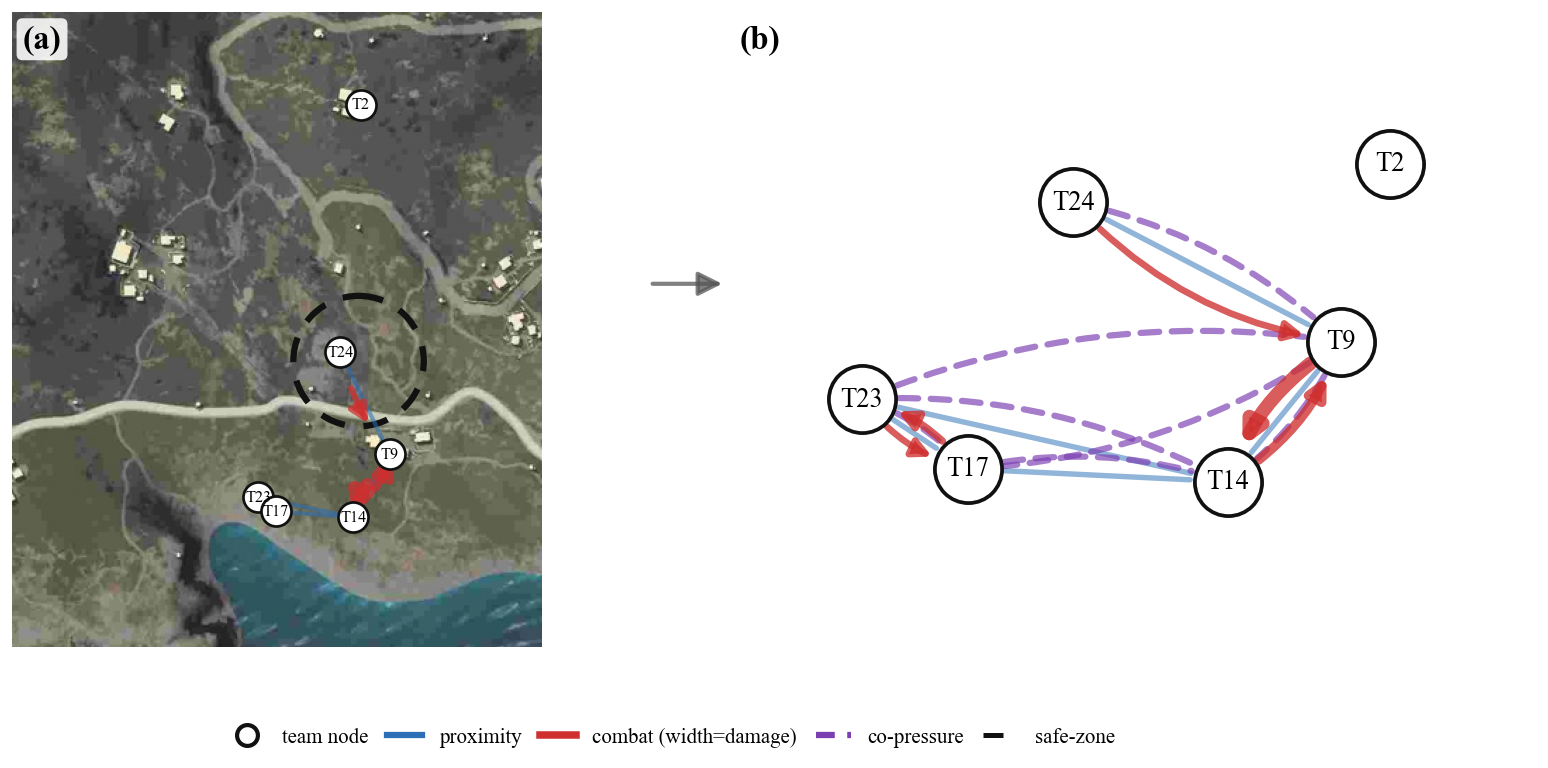
\includegraphics[width=0.78\textwidth]{figures/dynamic_heterogeneous_graph_example.png}
\caption{동적 heterogeneous graph 예시. 팀 centroid, 안전 구역 경계,
교전 이벤트를 포함한 phase-level STDB snapshot을 팀 사이의 근접, 교전,
공동 압력 관계로 변환한다.}
\label{fig:dynamic-graph-example}
\end{figure*}

\paragraph{위험 예측 문제와 모델.}
각 분석 페이즈의 종료 시점에서 아직 생존해 있고 다음 구간이 관측되는
팀만 위험 집합에 포함한다. \(b_k\)를 페이즈 \(k\)의 종료 시점,
\(T_i\)를 팀 \(i\)의 탈락 시점이라 하자. 이진 목표 변수는 다음과 같다.
\[
Y_{i,k}=\Ind\!\left\{b_k < T_i \leq b_{k+1}\right\}, \qquad
h_{i,k}=P(Y_{i,k}=1 \mid T_i>b_k, X_{i,\leq k}).
\]
즉 \(Y_{i,k}=1\)은 팀 \(i\)가 \(b_k\)까지 생존했지만 다음 페이즈가 끝나기
전에 탈락했음을 의미한다. \(b_k\) 시점에 이미 탈락한 팀, 패딩된 팀 슬롯,
다음 페이즈가 관측되지 않는 셀은 분석과 손실 계산에서 제외한다.

DynamicSTGNN은 팀-페이즈 특징의 시간 순서와 근접, 교전, 공동 압력 그래프의
시간 순서를 함께 입력으로 받는다. 모델은 각 팀의 시간적 변화와 팀 사이의
관계를 함께 요약한 뒤, 각 기준 페이즈마다 다음 구간 탈락 위험 점수를 출력한다.
구체적으로 \(X\in\mathbb{R}^{B\times T\times N\times F}\)와
\(A\in\mathbb{R}^{B\times T\times E\times N\times N}\)를 입력으로 받으며,
\(T=8\), \(N_{\max}=128\), \(F=66\), \(E=3\)이다. 입력층은 노드 특징을
64차원 상태로 사상하고, 두 개의 spatio-temporal block을 통과시킨다. 각
block은 gated causal temporal convolution, 관계별 graph aggregation, 두 번째
causal temporal convolution, layer normalization과 residual connection으로
구성된다. Temporal convolution은 phase \(k\)가 \(k\) 이후 정보를 보지 못하게
하고, 패딩 팀과 위험 집합에 속하지 않는 셀은 graph 집계와 손실 계산에서
mask한다.
